In diesem Abschnitt werden die einzelnen Strukturelemente und die Organisation des \ac{TTT} während einer typischen Mission erklärt. Dabei wird auf das Buddyteam, den Trupp, den Zug und die gesamte Struktur der Kräfte eingegangen.\\
Die Struktur lehnt sich dabei an das System der Bundeswehr sowie der Amerikanischen Streitkräfte an und wird im \ac{TTT} als 6 + 2 System so gelebt.\\
Ganz unten in der Hierarchie der Strukturelemente steht das Buddyteam, welches aus zwei Soldaten besteht. Sie bilden die kleinste, elementarste Einheit. Zwei oder mehr Buddyteams werden durch einen Truppführer koordiniert und bilden so einen Trupp. Zwei Trupps bilden wiederum einen Zug, der durch die Zugführung geleitet wird. Alle Züge und Elemente werden von den Anweisung seitens der Operativen Planung (\ac{OPL}) geleitet.  

\section{\acf{OPL} / \acf{HQ}}
\begin{wrapfigure}{r}{0.35\textwidth}
	%\vspace{-15pt}
	\centering 
	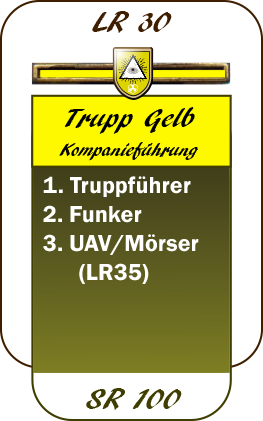
\includegraphics[width=0.3\textwidth]{../img/truppenordnung/opl/opl}
	%\caption{Beispiel einer \ac{OPL}}
	%\vspace{-30pt}
\end{wrapfigure}	

Die \ac{OPL} ist die höchste Instanz innerhalb einer Mission. Sie hat den Oberbefehl über alle Einheiten inne, koordiniert das allgemeine Vorgehen innerhalb der Mission und verwaltet die Zuordnung der unterstützenden Einheiten zu den kämpfenden Einheiten. Sie kommuniziert grundsätzlich nur über die Long-Range mit ihren untergeordneten Einheiten.\vspace{12pt}\\

Die \ac{OPL} ist folgendermaßen aufgebaut:
\begin{itemize}
	\item Operationsleiter\,/\,\acs{OPL} (\acf{CO}): Der Oberbefehlshaber der Mission. Er gibt die Befehle und erstellt "den großen Plan".
	\item stellv. \ac{OPL} (\acf{XO}): Unterstützt den \ac{OPL} bei seinen Aufgaben, typischerweise beim Funken mit den untergeordneten Trupps. Kann jedoch auch alle weiteren Aufgaben übernehmen, die ihm der \ac{OPL} überträgt -- er ist Mädchen für alles. Bewährt hat sich das Prinzip, dass der \ac{OPL} den eingehenden Funk übernimmt (Anfragen von anderen Trupps) und der stellv. \ac{OPL} den ausgehenden Funk (Abfragen von Statusberichten, Übermittlung von neuen Befehlen).
\end{itemize}
Ergänzt werden kann die \ac{OPL} durch maximal 4 Spieler, welche folgende Rollen einnehmen können:
\begin{itemize}
	\item Funker (\acf{RO}): ein zusätzlicher Funker, um die \ac{OPL} zu unterstützen, kann auf eine Spezialrolle beschränkt sein und für diese eine eigene LR-Frequenz bekommen (so kann es z.\,B. bei einer Mission mit vielen Lufteinheiten sinnvoll sein, jemanden zu haben, der sich auf einer eigenen Frequenz nur um die Koordination der Lufteinheiten um das Flugfeld kümmert und zentraler Ansprechpartner aller Lufteinheiten für Start-\,/\,Landemanöver ist)
	\item Aufklärungsoffizier (\acf{IO}): Sammelt alle verfügbaren, relevanten Daten und leitet diese gegebenenfalls an andere Trupps weiter. Hat meistens eine eigene, "große" Drohne (Greyhawk\,/\,Global Hawk) zur Feindaufklärung.
	\item freie Rolle (maximal einmal): je nach Mission kann es sinnvoll sein, dem \ac{OPL} einen Sanitäter, einen Nahsicherer, einen Fahrer o.\,Ä. zur Seite zu stellen
\end{itemize}
Je nach Größe und Struktur der Mission kann die \ac{OPL} identisch sein mit
\begin{itemize}
	\item der Sektionsführung, falls die Truppstruktur der Mission nur aus einer Sektion besteht
	\item der Zugführung, falls die Truppstruktur der Mission nur aus einem Zug besteht (egal ob Infanteriezug, Panzerzug oder mechanisierte Infanterie). Dies ist die einzige Ausnahme, in der die \ac{OPL} per Short-Range statt Long-Range mit ihren untergeordneten Einheiten kommuniziert.
\end{itemize}
Die OPL hält typischerweise einen sehr großen Abstand zu ihren Truppen - oft bleibt sie auch durchgehend in der Basis.

\section{Zugführung / Squadlead (SQL)}
\begin{wrapfigure}{r}{0.4\textwidth}
	\centering 
	\vspace{-20pt}
	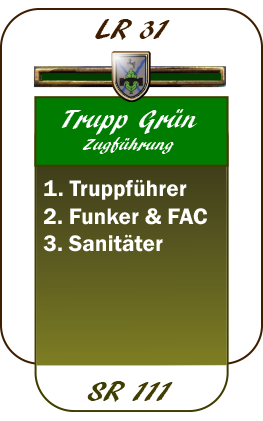
\includegraphics[width=0.3\textwidth]{./img/truppenordnung/zugfuehrung/zugfuehrung}
	%\caption{Beispiel eines \aclp{SQL}}
	\vspace{-50pt}
\end{wrapfigure}
Die Zugführung ist das Führungselement der Infanterie und Bindeglied zu den anderen Trupps. Einer Zugführung unterstellt sind typischerweise zwei, maximal drei Infanterietrupps, des weiteren kann ein Zug durch maximal einen Spezialtrupp mit klarer Aufgabenstellung unterstützt werden. Die Kommunikation zwischen dem Zugführer und der ihm untergeordneten Trupps erfolgt über Short-Range ohne Funkprotokoll über den sogenannten Zugkanal, die Kommunikation zu anderen Trupps über Long-Range.\\

Eine Zugführung besteht aus ein bis drei Spielern:
\begin{itemize}
	\item Zugführer\,/\,Squadlead (SQL)): Er befehligt die ihm untergeordneten Trupps. Ist kein Funker in der Zugführung vorhanden, übernimmt er auch die LR"=Kommunikation zu anderen Einheiten, in diesem Fall fällt jedoch die interne SR"=Truppfrequenz weg und der Zugfunk wird zum Standardfunk des Zugführers.
	\item Funker\,/\,Radio Operator (RO): Übernimmt die Kommunikation zu anderen Einheiten, damit der Zugführer sich auf die Führung seiner Truppen konzentrieren kann. Optional, wird jedoch dringend empfohlen.
	\item Gefechtssanitäter\,/\,Combat Medic (CM): Sanitäter für die Erstversorgung und Organisation der Verwundeten im Feld. Optional.
\end{itemize}
Sollten mehrere Züge im Verbund arbeiten, so einigen sich die Funker dieser Züge im Vorhinein auf eine sogenannte Task"=Force"=Frequenz, die sie sich auf der Additional"=Long"=Range einrichten und über die sie direkt ohne Funkprotokoll miteinander kommunizieren können (ähnlich wie der Zugkanal).\\
Die Zugführung sollte immer in Sichtweite der ihr unterstellten Trupps bleiben und sich maximal 200m bis 300m von ihnen entfernen, optimalerweise jedoch so nah wie möglich an ihren Truppen sein.
\section{Infanterietrupp / Fireteam (FT)}
\begin{wrapfigure}{R}{0.35\textwidth}
	\vspace{-50pt}
	\centering 
	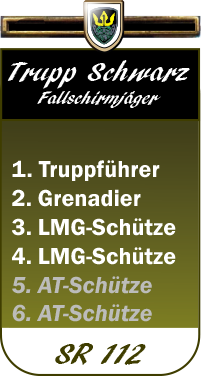
\includegraphics[width=0.2\textwidth]{../img/truppenordnung/infanterie/infanterie}
	%\caption{Beispiel eines Infantrietrupps}
	\vspace{-90pt}
\end{wrapfigure}
Die Infanterie bildet den Kernbestandteil vieler Missionen. Ein Infanterietrupp ist immer Teil eines Zuges und besteht aus 4 oder 6 Mann. Mögliche Positionen innerhalb eines Infanterietrupps sind:
\vspace{3.5cm}
\begin{longtable}{@{}P{0.4\textwidth}P{0.4\textwidth}@{}}
	\toprule
	Deutsche Bezeichnung & Englische Bezeichnung\\
	\midrule
	Truppführer (TF) & Fireteam Leader (FTL)\\
	Grenadier (GRE) & \\
	Leichter MG-Schütze (LMG) & Automatic Rifleman (AR)\\
	Mittlerer MG-Schütze & Medium Machine Gunner (MMG) \\
	MG-Assistent & Assistant Machine Gunner (AMG)\footnote{notwendig für MMG}\\ 
	Leichter Panzerabwehrschütze & Light Anti Tank (LAT)\\
	Schwerer Panzerabwehrschütze & Heavy Anti Tank (HAT)\\
	Panzerabwehr-Assistent & Assistant Anti Tank (AAT)\footnote{notwendig für HAT}\\ 
	Luftabwehrschütze & Anti-Air (AA)\\
	Pionier & Pioneer (PIO)\\
	Gefechtssanitäter & Combat Medic (CM)\\
	Schütze & Rifleman (RI)\\			
	\bottomrule					
\end{longtable}


Auf eine sinnvolle Einteilung in Buddy"=Teams (z.\,B. bei Positionen, die einen Assistenten erfordern), ist hierbei zu achten.\\
Die Kommunikation erfolgt ausschließlich über Short-Range, der Truppführer schaltet sich über seine Additional-Short-Range auf den Zugkanal auf, um sich mit der Zugführung und den anderen Truppführern im Zug abzusprechen. Die Nummer 2 im Trupp kann sich ebenfalls auf den Zugfunk aufschalten, jedoch nur mithören und nicht funken -- es sei denn, der Truppführer fällt aus und die Nummer 2 übernimmt.

\section{Spezialtrupp}

\includegraphics[width=20mm]{../img/truppenordnung/spezialeinheiten/sf1}\quad

\includegraphics[width=20mm]{../img/truppenordnung/spezialeinheiten/sf2}\linebreak
Spezialtruppen sind infanteristische Einheiten bestehend aus zwei bis sechs Mann mit einem klaren Aufgabenschwerpunkt -- dies kann vom klassischen Zwei"=Mann"=Scharfschützenteam bis zum Sechs-Mann-Kampftauchertrupp gehen. Sie sind die flexibelsten Einheiten innerhalb des TTTs und können entweder autark arbeiten oder im Verbund mit einem anderen Trupp oder Zug. Pro Mission existieren maximal zwei autark operierende Spezialtruppen, im Verbund mit einem Zug maximal einer.\par
Kommunikation erfolgt über Long"=Range, beim Arbeiten im Verbund zusätzlich über die Additional"=Short"=Range (Zugfunk). Kämpfende Einheiten wie z.B. Kommandotrupps oder Kampftaucher, in denen der Truppführer viel Mikromanagement leisten und der Trupp in direkte Feuergefechte verwickelt wird, benötigen zwingend einen separaten Funker. In unterstützenden Einheiten wie z.B. Aufklärungsteams oder Mörserteams, die voraussichtlich nicht in direkte Feuergefechte verwickelt werden, kann (muss aber nicht) der Truppführer die Long"=Range"=Kommunikation mit übernehmen.\par
Mögliche Aufgabenschwerpunkte eines Spezialtrupps sind z.\,B.:
\begin{itemize}
	\setlength\itemsep{0em}
	\item JTAC-Team
	\item Aufklärungsteam (UAV)
	\item Autonome Kampfeinheit (UGV)
	\item Mörserteam
	\item schwere Feuerunterstützung (Schweres Maschinengewehr (HMG) / Granatmaschinengewehr (GMG))
	\item (schwere) Panzerabwehr / Flugabwehr (falls nicht bereits im Zug vorhanden)
	\item Pionier-Team (falls nicht bereits im Zug vorhanden)
	\item medizinische Versorgung/Unterstützung (falls kein MedEvac in der Mission vorhanden)
	\item Kommandokräfte (Infiltration)
	\item Scharfschützenteam
	\item Kampftaucher
\end{itemize}
Bei entsprechenden Rollen (schwere Waffen, Mörser, etc.) ist auf das Vorhandensein eines entsprechenden Assistenten zu achten.
\section{Logistik}

\includegraphics[width=20mm]{./img/truppenordnung/logistikMedevac/TrSilber}\\
Silber -- Bussard -- Stellt Fahrzeuge und Personal bereit, mit denen Transport und Logistik durchgeführt werden.
\section{MedEvac}

\includegraphics[width=20mm]{../img/truppenordnung/logistikMedevac/weiss}\linebreak
Weiß -- \acf{MedEvac} -- Unterstützt Operationen mit Versorgungs- und Transportkapazität für Verwundete.
\section{Close Air Support}

\includegraphics[width=20mm]{../img/truppenordnung/logistikMedevac/silber}\\
Silber -- Adler -- Stellt Fahrzeuge und Personal bereit,  Gefechtsunterstützung (\ac{CAS}) und Geleitschutz durchgeführt werden.
\section{Mechanisierte Infanterie}
Das Konzept der mechanisierten Infanterie befindet sich im Moment noch in Arbeit und wird in einer späteren Version des Handbuches hinzugefügt.
\section{Kampfpanzer}
Das Konzept der Kampfpanzer befindet sich im Moment noch in Arbeit und wird in einer späteren Version des Handbuches hinzugefügt.
\section{Artillerie}
Das Konzept der Artillerie befindet sich im Moment noch in Arbeit und wird in einer späteren Version des Handbuches hinzugefügt.